\section{Results}
\label{sec:rslts}

%introduction

\subsection{Clustering Results}
\label{ssec:clures}
\mynote[author=Harrie]{Je verhaal is moeilijk te volgen omdat de resultaten die je bespreekt in de appendix staat, zet de belangrijke resultaten in de text. (Hyperparameters horen wel in de appendix.)}
In this part the results for clustering both the user and job features is described.
The first attempt is to cluster the user or job data using the K-prototypes algorithm which can deal with both numerical and categorical data. 
To improve the clustering results the numerical data is converted to \textit{z}-scores.
When this algorithm is applied the clustering time after time breaks down around cluster size 50, when the algorithm fails to initiate the cluster centroids. 
Diverse cluster initiation schemes and even manual initiation have been tried, but the problem persists. 

Due to the fact that the K-prototypes could not be used and because of the fact that only a few columns were numerical it was decided to treat all numerical data as categorical data and to apply the K-modes algorithm.
For the users optimal cluster size seems to be around 150 and for jobs around 100 (figure \ref{fig:eb})
However, the elbow plots do not show a determinative point where they flatten out.
Thus to validate the clustering results the cluster sizes 25 till 300 with an interval of 25 were tested on 12 scenarios (appendix \ref{ssec:cluscen}) for both Logistic Regression and Neural Network.
Even though in total 288 tests were  conducted (12$\times$12$\times$2) the results did not show any improvement in the prediction objective. 
Therefore, the clustering method cannot be applied for the recommender system.

\begin{figure}[H]
    \centering
    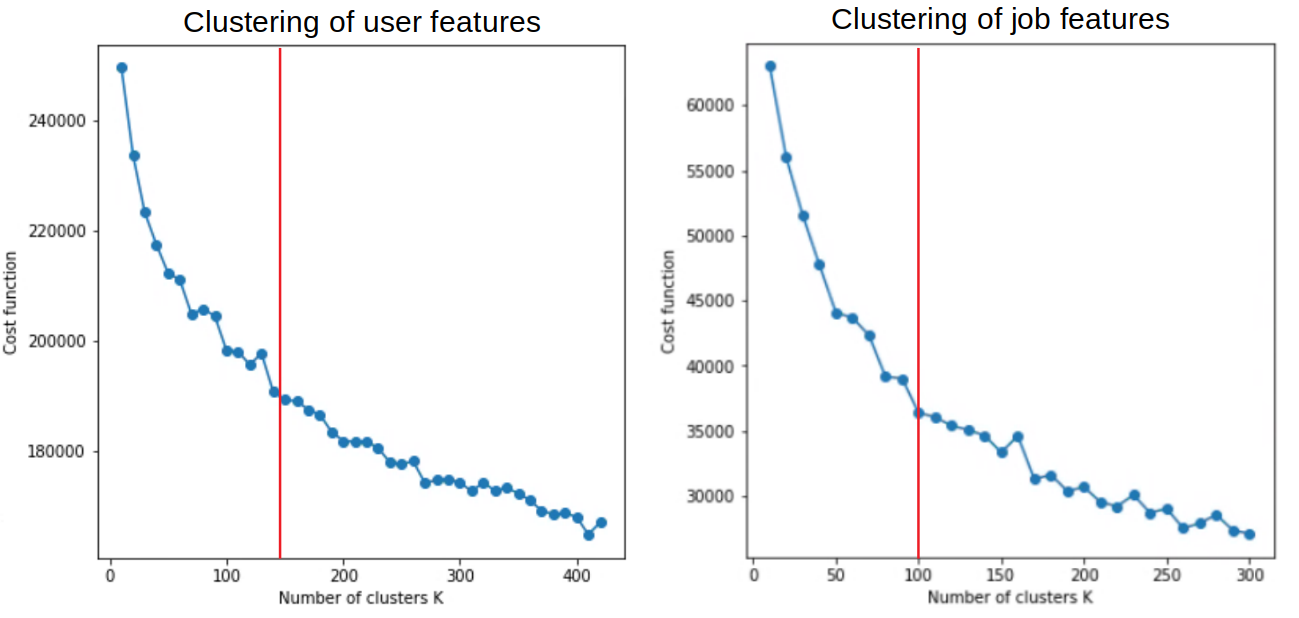
\includegraphics[width=\linewidth]{ThesisTemplate/Images/Clustering.png}
    \caption{\label{fig:eb} Elbow plots users and jobs clustering}
\end{figure}

% \begin{table}[h]
% \begin{footnotesize}
% \begin{tabular}{llll}
\toprule
\textbf{Scenario}   & \textbf{\# clusters}  & \textbf{Accuracy} & \textbf{MCC}    \\
\midrule
1                   & 225                   & 0.81              & 0.41            \\ %6.7
2                   & 275                   & 0.82              & 0.49            \\ %6.15
3                   & 300                   & 0.75              & 0.08            \\ %6.8
4                   & 100                   & 0.77              & 0.05            \\ %6.13
5                   & 225                   & 0.82              & 0.45            \\ %6.2
6                   & 300                   & 0.77              & 0.27            \\ %6.3
7                   & 250                   & 0.84              & 0.55            \\ %6.14 
9                   & 150                   & 0.79              & 0.27            \\ %6.12
10                  & 25                    & 0.15              & 0.11            \\ %6.4
11                  & 25                    & 0.93              & 0.92            \\ %6.6
12                  & 25                    & 0.11              & 0.05            \\ %6.10 
13                  & 25                    & 0.89              & 0.88            \\ %6.11
\bottomrule
\end{tabular}
% \end{footnotesize}
% \caption{\label{tab:clures} Best Results Clustering}
% \end{table}

\subsection{Results Content-Based Learning Models}
\mynote[author=Harrie]{Een confusion matrix zou hier heel goed werken, of anders iets van (percentage) false/true positives/negatives, omdate de MCC toch moeilijk te interpreteren is.}
When assessing the accuracy results it must be taken into account that the dataset exhibits a class imbalance of 79\% being positive labels and 21\% being negative labels. 
The consequence of this imbalance is that if the classifier predicts all labels to be positive it achieves 0.79 accuracy. 
This fallaciously suggests that the classification results are decent.
Here is where the utility of the Matthews correlation coefficient (MCC) comes into play, as the MCC in such case will be 0.00 because no labels are classified as negative. 

The classification results of the models are shown in table \ref{tab:res}.
For training and validation of all models a fixed split of 80/20 is used.
Judging only on the accuracy alone it does not seem to make a great difference which model is applied.
When the MCC scores are analyzed the Neural Network performs 10\% better than its closest rival and 52\% better than the baseline. 
The higher performance of MCC suggests better balanced predictions of both the positive and negative labels.
The best scores for the Neural Network were achieved with a setup of one hidden layer. 
When more hidden layers are added the performance decays gradually.
The more hidden layers the more complex patterns the Neural Network can learn, on the other hand this also increases the chance of overspecialization (overfitting) on the train data. 
Therefore, it can be argued that when extra layers are added the performance is worsens due to overfitting. 

\begin{table}[h]
\begin{footnotesize}
\begin{tabular}{lrr}
\toprule
\textbf{Model}      & \textbf{Accuracy} & \textbf{MCC}  \\
\midrule
Nearest Neighbors (baseline)   & 0.76              & 0.29          \\     
K-Nearest Neighbors & 0.80              & 0.35          \\
RandomForest        & 0.82              & 0.40          \\
Logistic Regression & 0.80              & 0.35          \\
Linear SVC          & 0.80              & 0.33          \\
Neural Network      & 0.81              & 0.44          \\
\bottomrule
\end{tabular}

\end{footnotesize}
\caption{\label{tab:res} Training Results Models}
\end{table}

The MCC score is low and therefore also the precision, recall and F-measure were analyzed.
Overall the performance of all models is good on predicting the positive labels and bad when it comes to predict the negative labels.
Due to the class imbalance the classifiers display a tendency to overpredict the positive labels, and therefore it is hard to determine how well the positive labels are learned. 

\begin{table}[h]
\begin{footnotesize}
\begin{tabular}{l|l|l|r|r|}
    \multicolumn{3}{c}{\multirow{2}{*}}                          &  \multicolumn{2}{c}{\textbf{Actual labels}}   \\ 
    \cline{4-5}
    \multicolumn{3}{c|}{}                                        &Positive           &Negative                   \\
    \cline{3-5}
    \multicolumn{2}{l|}{\textbf{Predicted}}  &Positive           & 1,129      &111                  \\
    \cline{3-5}
    \multicolumn{2}{l|}{\textbf{labels}}     &Negative           & 190         &181                 \\
    \cline{3-5}
\end{tabular}





\end{footnotesize}
\caption{\label{tab:cmnn} Confusion Matrix Neural Network}
\end{table}

\begin{table}[h]
\begin{footnotesize}
\begin{tabular}{lrrrr}
\midrule
\textbf{Label}      & \textbf{Precision} & \textbf{Recall}  & \textbf{F1-score}    & \textbf{Support}    \\
\midrule
Positive            & 0.86               & 0.91             & 0.88                  & 1,240        \\
Negative            & 0.62               & 0.49             & 0.55                  & 371        \\
\midrule
\end{tabular}



\end{footnotesize}
\caption{\label{tab:crnn} Classification Report Neural Network}
\end{table}

\subsection{Ranking Results}
Another method to evaluate the classification of the positive labels is by ranking them and then retrieving the average rank.
To achieve that the train model predicts the label probability of each user-job combination, whereafter the average rank can be calculated.
There are 4,983 unique jobs (midpoint is 2,491), and the expectation would be that the positive labels would at least come in the top 100. 
The results show a different picture, for Logistic Regression the average rank of the positive labels is 2,611 and for the Neural Network 2,250.
The Neural Network performs best, but the results are not significant better than the random selection and definitely not close to an average rank below 100.



%logistic regression ranks the jobs for all users the same

%K-modes - descent, but no better learning results when predicting cluster or when added as extra feature
%hierarchical - good results on visual inspection, but no better learning results when predicting cluster or when added as extra feature (check this!)

% \todo{Content based Models}
% Neural network
    % One layer setup works best (assumption of overfitting when more layers are added)
% Logistic Regression
    % Ranking: same rankings for every user, because per row the user is the same and only the jobs are different
% Ranking
    % Random outcomes
    % validated by overfitting on subsample, predicted all 1

\todo{Strategies to improve}
% Under-oversampling worsen results
% Feature importance slight improvement of results
